\chapter{Projektplanung}
\label{sec:Projektplanung}
\index{Projektplanung}

%-------------------------------------------------------------------------------------------------------------------
\section{Gantt Chart}
\index{Gantt Chart|(}
F�r die Projektplanung wurde ein Java-Tool benutzt, welches auf dem Gantt-Diagramm basiert. Es ist unter dem Namen \href{http://www.ganttproject.biz/download}{GanttProject} \footnote{offizielle Website \url{http://www.ganttproject.biz}} bekannt.\\
Ein Gantt-Diagramm oder Balkenplan ist ein nach dem Unternehmensberater Henry L. Gantt (1861-1919) benanntes Instrument des Projektmanagements, das die zeitliche Abfolge von Aktivit�ten grafisch in Form von Balken auf einer Zeitachse darstellt.\\
Der Vorteil des Gantt Chart besteht darin, dass die Aktivit�tedauer durch die Balkenl�nge wiedergegeben wird. Eine Ende-Start-Beziehung kann auch im Verlauf einer Aktivit�t ansetzen.\\
Der Nachteil liegt darin, dass Abh�ngigkeiten zwischen einzelnen Aktivit�ten nur zeitbezogen dargestellt werden k�nnen.\\
Es gibt viele kostenlose sowie kostenpflichtige Software, die mit Gantt Chart arbeiten. Das wohl bekannteste lizenzpflichtige Programm ist das \href{http://office.microsoft.com/de-ch/visio}{Microsoft Visio} \footnote{\url{http://office.microsoft.com/de-ch/visio}} oder \href{http://www.microsoft.com/project/en-us/Preview}{Microsoft Project} \footnote{\url{http://www.microsoft.com/project/en-us/Preview}}.
Quelle: \cite{gantt_chart} und \cite{gantt_project}

\begin{figure}[h!]
\centering
\noindent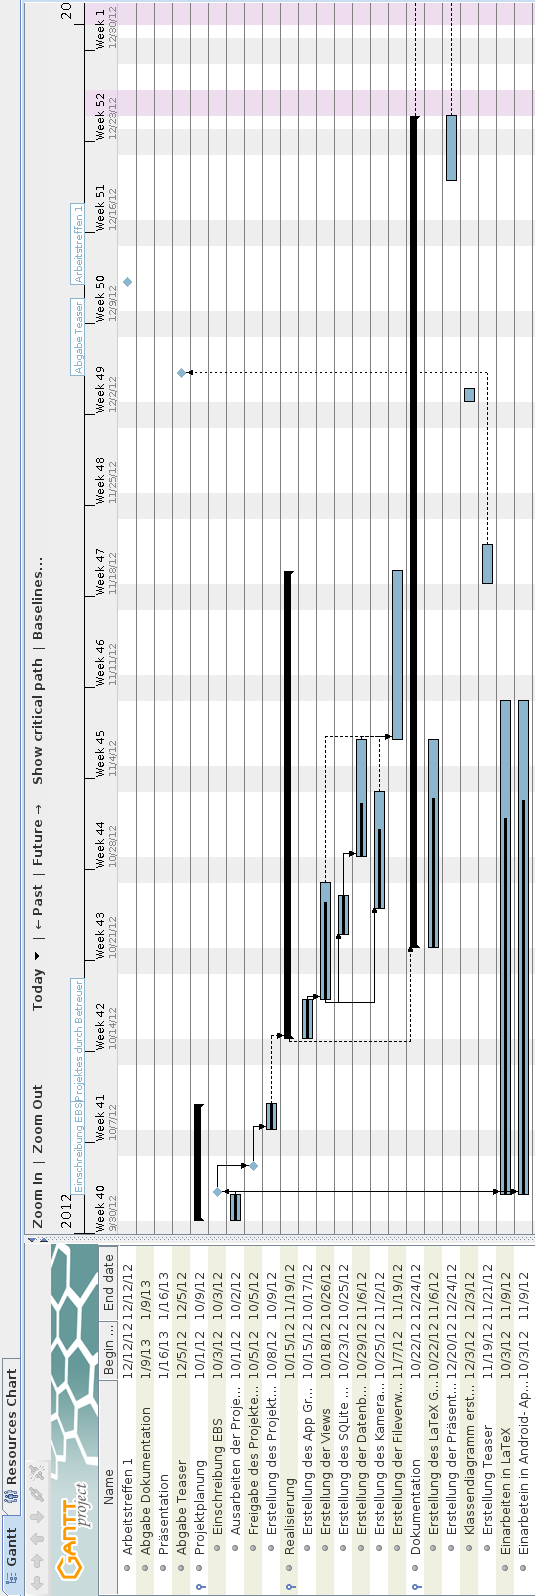
\includegraphics[height=0.85\textheight]{gantt_chart.png} 
\caption{Gantt Chart Projekt Warranty}
\label{Gantt_Chart}
\end{figure}
\index{Gantt Chart|)}


%-------------------------------------------------------------------------------------------------------------------
\section{Arbeitsaufw�nde}
\begin{tabular}[t]{|l|c|c|} \hline
\cellcolor{darkgrey} &  \cellcolor{darkgrey} &  \cellcolor{darkgrey}\\
\cellcolor{darkgrey} \multirow{-2}{5cm}{\textbf{Bezeichnung}} &
\cellcolor{darkgrey} \multirow{-2}{3cm}{\textbf{Aufwand gesch�tzt [h]}} &  
\cellcolor{darkgrey} \multirow{-2}{3cm}{\textbf{Aufwand effektiv [h]}}  \\ \hline

\multicolumn{3}{|l|}{} \\
\multicolumn{3}{|l|}{\multirow{-2}{5cm}{ \textbf{Projektplanung} }} \\ \hline
Ausarbeitung Projekdetails & 4 & 6 \\ \hline
Erstellung Projektplanes & 2 & 3 \\ \hline

\multicolumn{3}{|l|}{} \\
\multicolumn{3}{|l|}{\multirow{-2}{5cm}{ \textbf{Realisierung I} }} \\ \hline
Grundger�st Applikation  & 11 & 11\\ \hline
Views & 9 & 9\\ \hline
SQLite DB Schemas & 3 & 3\\ \hline
Datenbank Methoden & 6 & 3\\ \hline
Kamerasupports & 7  & 7\\ \hline
Fileverwaltung & 4 & 4\\ \hline


\multicolumn{3}{|l|}{} \\
\multicolumn{3}{|l|}{\multirow{-2}{5cm}{ \textbf{Realisierung II} }} \\ \hline
DB Zugriffe �berarbeiten  & 4 &  4\\ \hline
File und Fotoverwaltung �berarbeiten & 3 & 3\\ \hline
Views �berarbeiten  &3 &  3\\ \hline
Code Cleanup & 5 &  5\\ \hline

\multicolumn{3}{|l|}{} \\
\multicolumn{3}{|l|}{\multirow{-2}{10cm}{ \textbf{Dokumentation und Pr�sentation} }} \\ \hline
Erstellung Teaser  & 3 & 2 \\ \hline
Erstellung Logo& 3 & 2 \\ \hline
Erstellung LaTeX Grundger�st  & 10 &  23\\ \hline
1. Einleitung  & 3 &  3\\ \hline
2. Projektplanung  & 3 & 3 \\ \hline
3. Grundlagen App Programmierung & 10 &  10\\ \hline
4. Warranty App & 4 & 8 \\ \hline
5. Fazit & 2 &  2\\ \hline
Anhang & 4 &  3\\ \hline
Klassendiagramm & 3 &  5\\ \hline
Erstellung Javadoc& 5 &  5\\ \hline
Erstellung Pr�sentation & 12 &  8\\ \hline

%\multicolumn{3}{|l|}{} \\
%\multicolumn{3}{|l|}{\multirow{-2}{10cm}{ \textbf{Diverses} }} \\ \hline
Einarbeitung in LATEX  & 15 & 26 \\ \hline
Einarbeitung Android Programming & 12 & 20 \\ \hline

&  &  \\
\textbf{Total Stunden}  & 
\textbf{150}&
\textbf{185}
\\ 

&  &  \\ \hline

\end{tabular}\\



